\section{Aufbau}
Zentrales Element des Aufbaus ist ein Helium-Neon Laser der mit einer Wellenlänge von $\lambda = 633\si{\nano \meter}$ auf einen
verschiebbaren Spalt strahlt. Auf Grund der langen Kohärenzlänge von Lasern ist der Abstand zum Spalt ohne Bedeutung.
Das vom Spalt erzeugte Inteferenzmuster wird anschließend auf einen Lichtempfindlichen Detekor projeziert, 
welcher in der Lage ist, durch eine Photoiode, die Intensität festzustellen. Der Abstand zwischen dem Spalt und 
dem Detekor misst $127\si{\cm}$. 
\\
\newline
Der Spalt wird auf eine Halterung unmittelbar hinter dem Laser angebracht und so ausgerichtet, dass der Lichtstrahl 
genau durch den zum Verusch passenden Aufbau läuft. Für den Versuch werden zwei Konfiguartionen der Spalte benutzt, wobei der 
einfacher Spalt einer Breite von $b_{\text{einfach}}=0.075 \si{\mm}$ misst.
\\
\newline
Um die Maxima und Minima des Inteferenzmusters ablesen zu können, ist der Detekor auf eine Schiene montiert und anschließend an ein 
Ampermeter angeschlossen. 
Diese Schiene bietet eine Variation von jeweils $25 \si{\mm}$ nach oben und unten und ermöglicht es so die vom Winkel
$\varphi$ abhängige Intensität zu messen.
\begin{figure}
    \centering
    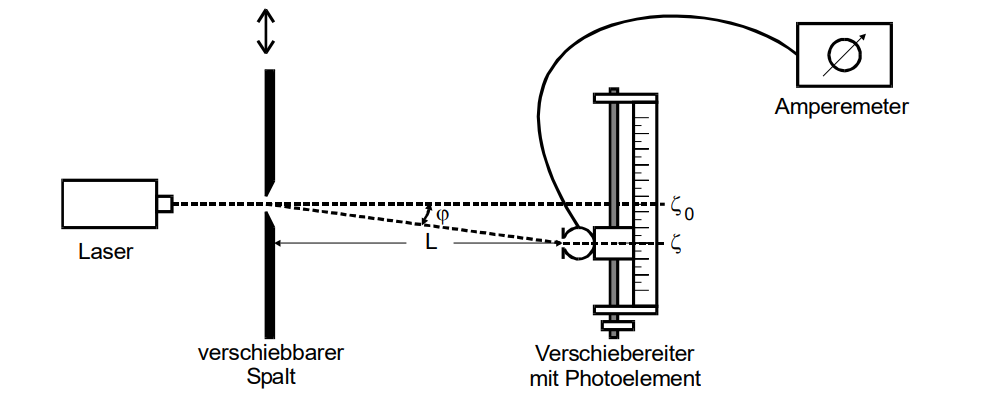
\includegraphics[width=\textwidth]{bilder/aufbau.png}
    \caption{Schematischer Aufabu des Lasers mit verschiebbaren Spalt und Detekor \cite{skript}.} 
    \label{fig:abb1}
\end{figure}
\section{Durchführung}
Zu Beginn des Versuches wird der vom Ampermeter gemessene Dunkelstrom festgestellt, um ihn von den folgenden Messungen abzuziehen.
Dafür wird der Raum best möglich verdunkelt und das Ampermeter ohne Lichtquelle eingeschaltet.
\\ 
\newline
In der ersten Messreihe werden die Werte für den einfachen Spalt entnommen. Dafür wird der Detekor solange verschoben, biss das erkennbare Hauptmaximum 
gefunden ist. Aus dieser Postion wird die Volle Variation der verschiebaren Schiene ausgenutzt und im Abstand von $-25 \si{\mm}$ bis 
$25 \si{\mm}$ vom Hauptmaximum die Intensität in 50 einzelnen Messschritten gemessen. 
Hierbei wird durch kleinere Intervalle besonders auf den Bereich um das Hauptmaximum geachtet.
\\
\newline
Die zweite Messreihe wird analog zur ersten Messung ausgeführt, mit Wechsel vom einfachen - zum Doppelspalt.
Hierbei gilt es vorab wieder das Hauptmaximum zu finden und anschließend in 50 Messungen die Intensität, abhängig vom Winkel,
abzulesen. 